\documentclass[12pt,a4paper]{report}
\usepackage[utf8]{inputenc}
\usepackage[spanish]{babel}
\usepackage{amsmath}
\usepackage{amsfonts}
\usepackage{amssymb}
\usepackage{makeidx}
\usepackage{graphicx}
\usepackage[hidelinks]{hyperref}
\usepackage[left=2cm,right=2cm,top=2cm,bottom=2cm]{geometry}
\usepackage{hyperref}



\begin{document}

\author{Cesar Omar Alvarado Contreras\\
Marco Manzo Torrez\\
Eduardo Robles Vazquez\\
Victor Gabriel Tapia Casillas\\
Fonseca Camarena Jonathan}

\title{\begin{center}

\includegraphics[scale=1.5]{Escudo.png} 
\end{center}Brazo Robótico Polar}

\date{
Universidad Politécnica de la Zona Metropolitana de Guadalajara\\
Profesor: Carlos Enrique Morán Garabito\\
17 de octubre 2019}

\maketitle
\tableofcontents
\section{Meta:}
Crear un robot polar de tres grados de libertad, con una longitud total de 50 centímetros y una altura total de 30 centímetros, cuyo último eslabón deberá soportar una carga de 500 gramos.
\section{Objetivos:}
\noindent
-Realizar boceto\\
-Cumplir con las especificaciones propuestas por el profesor\\
-Realizar el plano del robot\\
-Realizar el modelado del prototipo en 3D\\
-Establecer los materiales a usar\\ 
-Realizar el análisis de elementos finitos\\
-Realizar cálculos necesarios para la selección de motores y componentes\\
-Elaboración del primer prototipo\\
-Programación del robot\\



\section{Justificación}
El propósito de este proyecto surge a partir de la necesidad de implementar los conocimientos obtenidos de las materias presentes en este año, así como las materias de cuatrimestres pasados.
Retomando lo mencionado con anterioridad, se desarrollará un prototipo de un brazo robótico polar, el cual consistirá de 3 grados de libertad; dos movimientos rotacionales y uno prismático.

\section{Tabla de materias}
A continuación presentamos la tabla de materias que nos ayudarán en nuestro proyecto.\\
\begin{center}
\includegraphics[width=16cm]{tabla.png}
 Figura 1: Tabla 
\end{center}



\section{Project}
En el programa Project realizamos el cronograma de actividades.\\

\begin{center}
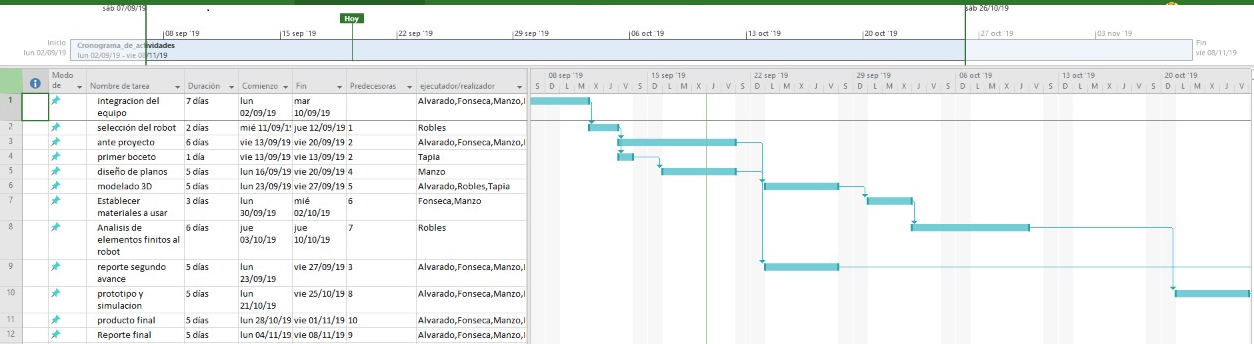
\includegraphics[width=18cm]{Project.png}
   Figura 2:Project
    
\end{center}



\section{Proposición del análisis finito}
El objetivo en este segundo avance es proponer fundamentar en actividad el estudio de mecanismos del robot.\\
Lo que se pretende calcular del robot, es la cantidad que puede soportar, esperando como resultado una carga de 500gramos, calcular los diámetros correspondientes a los pasadores para evitar cargas por cortante; selección del material para la estructura y actuadores, como también el calculo de estimación del tiempo de vida del robot.\\

\section{Material seleccionado}

Para darle una mayor resistencia a la estructura del robot se planea utilizar una aleación de aluminio, ya que tiene mayor resistencia al desgaste y deformación a diferencia de otros materiales además de ser relativamente ligero.\\


\begin{center}
\includegraphics[width=10cm]{tablaaluminio.png}
 Figura 3: Tabla Aluminio
\end{center}
Posteriormente se realizará una prueba de elementos finitos mediante un software para sustentar la idea de dicho material.\\

\section{Cronograma de gastos de elaboración de robot esférico}
 
\begin{center}
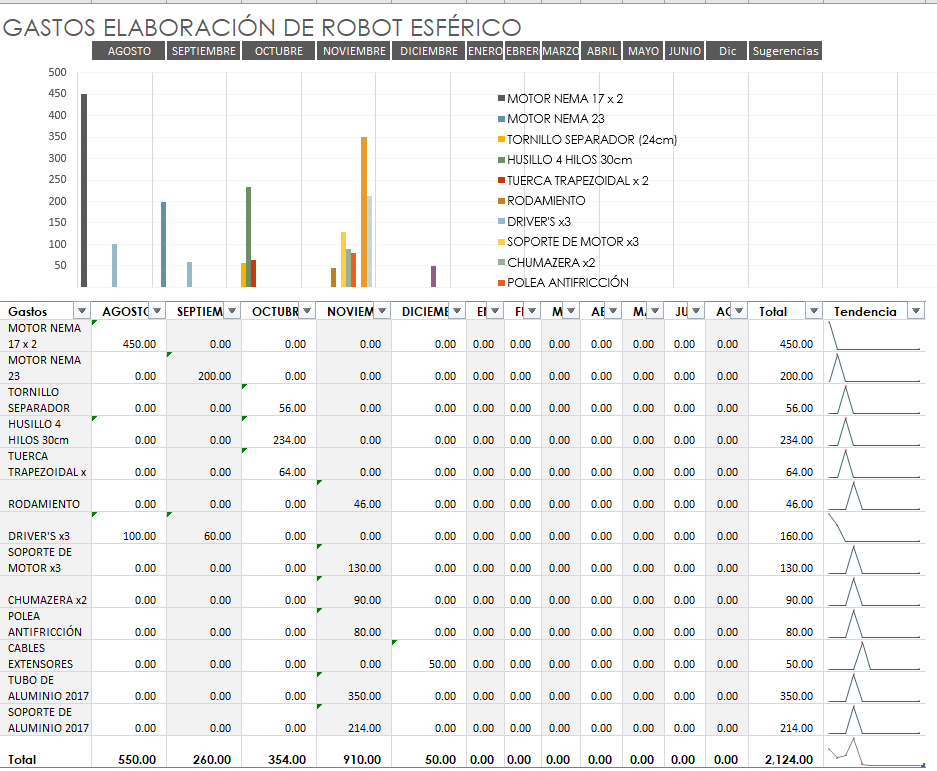
\includegraphics[width=16cm]{2019-10-18.png}
 Figura4 :Gastos de elaboración
\end{center}
    

\section{Avances en inventor}
El profesor Norberto Garcia principalmente nos aporto los conocimientos del diseño gráfico, problematicas, materiales resistentes (como madera, plásticos o metales) y sistemas y control (que incluye electrónica, control por ordenador y sistemas mecánicos) de proyectos anteriores que a observado.\\
\begin{center}
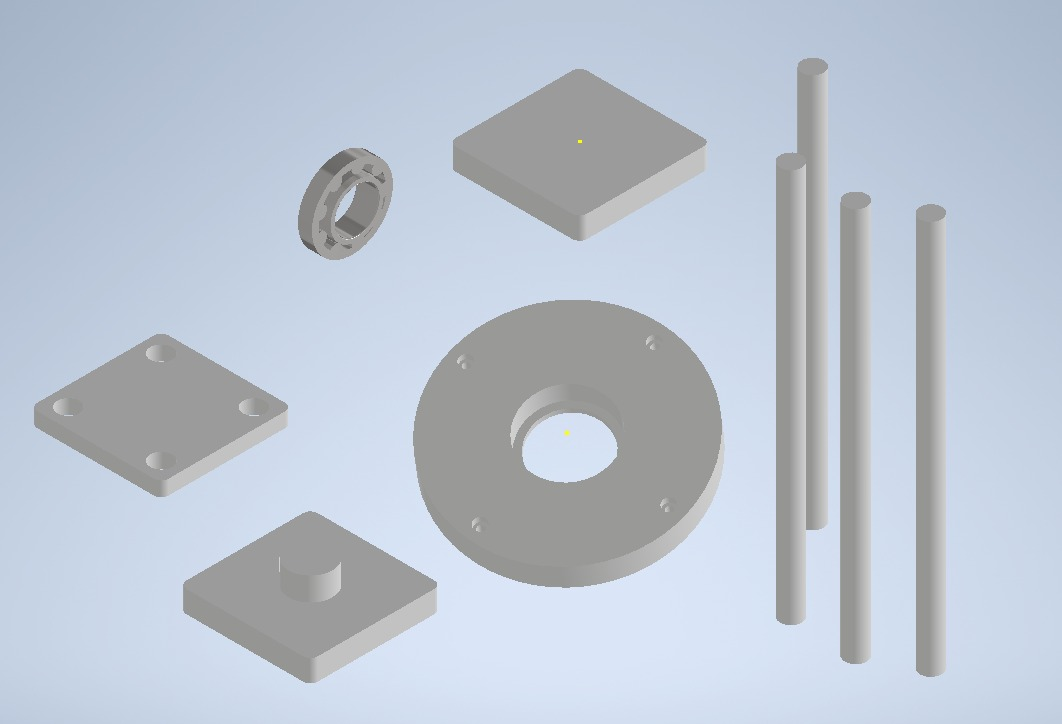
\includegraphics[width=5cm]{Dibujo1.jpeg}
 Figura 5:Dibujo1
\end{center}
Fue necesario realizar los dibujos barias ocaciones por que encontraba algun problema ya sea de medida o de fricción en las piezas de nuestro proyecto.\\
\begin{center}
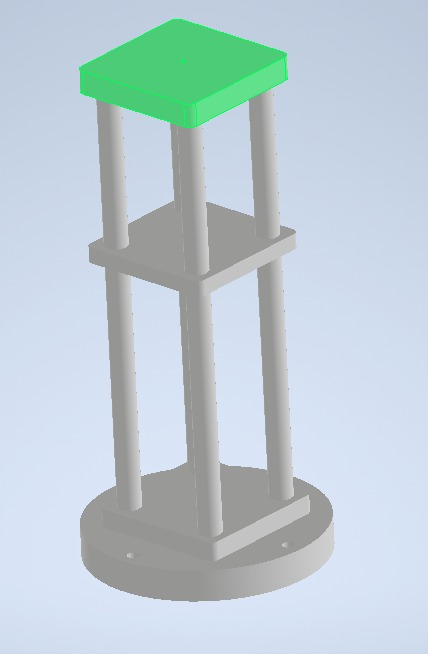
\includegraphics[width=5cm]{Dibujo2.jpeg}
 Figura 6:Dibujo2
\end{center}
Asimismo entedimos cómo convertir una idea de diseño en un producto real, eligiendo la mejor opción en cuanto al enfoque, las técnicas y los materiales a utilizar. Nuestro proyecto se emplea en el diseño asistido por ordenador (CAD) para llevar a término este proyecto.









  
\section{Conclusiónes}
Victor Gabriel Tapia Casillas: El proyecto va avanzando conforme lo planeado, ya se pasó de burdos bocetos en el cuaderno a modelos tridimensionales por software, nuestro siguiente paso a realizar es el análisis dimensional con el cual concluiremos con la selección de materiales y posteriormente se pasará al armado y programación del susodicho para empezar las pruebas previas a la entrega.\\

Marco Manzo Torrez: Es muy importante, desde que se comienza un proyecto, tener una idea clara de lo que se quiere realizar y la función que se quiere satisfacer. Cosas tan sencillas como la selección de un material, de un motor, de un mecanismo son las cosas que marcan la diferencia y que hacen posible la viabilidad de un proyecto. En este caso aunque nuestro proyecto aún no está terminado, va por un buen camino, va avanzando y cada vez se ve con una mayor perspectiva el trabajo aplicado en la construcción y el desarrollo.\\

Robles Vázquez Eduardo: En este avance hemos progresado según lo planificado, teniendo presente el modelado tridimensional de nuestro robot. Pará la siguiente etapa desarrollaremos el análisis de elementos finitos con el cual veremos y pondrémos a prueba el material que planeamos usar, para tener una idea de que tan resistente o bueno será para el proyecto. También llevaremos acabo un modelado matemático del comportamiento de los motores el cual nos ayudará a desarrollar mejor el proyecto.\\

Cesar Omar Alvarado Contreras: El proyecto de en si sigue un rumbo pero con varias brechas para tomar en cuestiones de sistemas implementados e igualmente solo se puede decir que el objetivo aun sigue en pie el cual esta definido en el tema visto, el problema que se ve es el diseño de la estructura ya que en ambos diseños provistos son robustos, e cada uno tiene su ventaja y desventaja como era de esperarse pero se opta por el segundo diseño que es mas practico y simple de elaborar y mas ligero.\\

Fonseca Camarena Jonathan: El diseño funcional del robot debe reflejar de manera general el funcionamiento del robot, debido a que es el punto del cual se empieza a identificar y desarrollar las partes del robot según su aporte para el funcionamiento del sistema final.
La selección del tipo de motores a emplear debe estar acorde a las necesidades, tanto de espacio, tipo de señal, sensibilidad, precisión, etc.\\
Para esto es necesario recurrir alas diferentes materias del cuatrimestre y preguntar en cada especialidad aportes y consejos que se podrian emplear en nuestro proyecto. Creo que para que un proyecto funciones es necesario la participación de los maestros de nuestra carrera.


\section{Referencia}

  E.F. Morales and L.E. Sucar,Los Robots del Futuro y su Importancia para M\'exico, Komputer Sapiens,
  year{2009},pages{7-12}


\bibliographystyle{unsrt}
\bibliography{Morales.bib}




\begin{center}
Gracias.
\end{center}


\end{document}